% MLSys 2027 submission draft.
% FORMAT: the official template is the MLSys 2025 style (mlsys2025style.zip from
% mlsys.org). This draft uses a plain two-column article so it compiles anywhere;
% before submitting, replace the preamble below with the official one
% (\usepackage{mlsys2025} etc.) and re-check the 10-page limit.
\documentclass[10pt,twocolumn,letterpaper]{article}
\usepackage[margin=0.75in,columnsep=0.25in]{geometry}
\usepackage{times}
\usepackage{amsmath,amssymb,amsthm}
\usepackage{graphicx}
\usepackage{booktabs}
\usepackage{xcolor}
\usepackage{hyperref}
\usepackage[capitalise]{cleveref}
\usepackage{natbib}

\newtheorem{proposition}{Proposition}
\newcommand{\TODO}[1]{\textcolor{red}{[TODO: #1]}}
\graphicspath{{../research/figures/}}

\title{Do Learned Load Balancers Herd?\\
\large Stale Shared State, Many Gateways, and Learned Power-of-$d$ Routing}
% Double-blind: no author names, affiliations, acknowledgements or
% identifying repository links in the submitted version.
\author{Anonymous Authors}
\date{}

\begin{document}
\maketitle

\begin{abstract}
Request routers in production are horizontally scaled: many gateway replicas
route independently using the same, slightly stale view of backend load, and
increasingly they score backends with learned latency models. Classic queueing
results show that shortest-queue routing on stale shared information
\emph{herds}: every dispatcher sees the same best server and they stampede onto
it. We ask whether learned routers inherit this failure, and what prevents it.
We simulate 12{,}630 runs and validate on a multi-process prototype. Routing
to the backend with the best learned prediction herds \emph{worse} than
classic shortest-queue routing. With 16 gateways and 50\,ms-stale state, its
P99 latency is 1.1\,s against 0.8\,s, and at 200\,ms it is 12.5\,s against
3.1\,s. Randomising gateway refresh phases rescues the classic policies but
not the learned one at scale: it still reaches 7.0\,s with 64 gateways.
Publishing routing weights on a control interval, a common design for learned
routers, is itself a hidden source of staleness. Combining learned latency
scores with power-of-$d$ candidate sampling bounds herding by construction.
Without any probing, its steady-state P99 stays between 108 and 282\,ms in
all 28 combinations of staleness, gateway count and refresh phase we tested. With $d{=}3$ live probes,
it matches an oracle that knows every server's true speed (84 vs.\ 83\,ms).
Under an unannounced gray failure it beats that oracle (112 vs.\ 206\,ms) and a
Prequal-style prober at the same probe budget (112 vs.\ 144\,ms).
\end{abstract}

% ---------------------------------------------------------------------------
\section{Introduction}

Every request to a large online service passes through a routing tier that
decides which backend replica serves it. That tier is itself a distributed
system: tens to hundreds of gateway or sidecar replicas sit behind an L4 load
balancer, and each decides on its own. Because backends cannot be polled on
every request, gateways share a periodically refreshed view of backend load
(e.g.\ heartbeats written to a key-value store) and route on that.

Two trends meet in this layer. First, routing decisions are increasingly
\emph{learned}: bandit-based and model-based routers predict per-backend latency
from context and route to the predicted best backend, and LLM-serving routers
score replicas by predicted cache reuse and load~\citep{llmd,vllmrouter,lodestar2026}.
Second, these routers are deployed as \emph{many independent replicas}, each
with its own model trained on the traffic it happened to see.

Queueing theory has long warned that combining the two ingredients of this
setting, stale shared information and many dispatchers, is dangerous.
Join-the-shortest-queue (JSQ) on old information causes \emph{herding}: all
dispatchers agree on the currently shortest queue and flood it until the next
update~\citep{mitzenmacher2000old,dahlin2000stale}. Randomised power-of-two
choices is the classic antidote~\citep{mitzenmacher2001power}. It is not known
whether learned routers, which add a second, slower feedback loop (the model),
behave like JSQ, better, or worse.

\paragraph{This paper.} We study herding in horizontally scaled learned
routers and make four contributions:
\begin{enumerate}
\item \textbf{Characterisation.} Argmin routing on learned latency predictions
  herds \emph{worse} than classic JSQ under stale shared state
  (\cref{sec:eval-herding}). Unlike JSQ, it is not fixed by desynchronising
  gateway refresh phases once there are many gateways, and it is catastrophic at
  high staleness. Publishing routing weights on a control interval, as
  learned-router designs commonly do, adds staleness of its own
  (\cref{sec:eval-epoch}).
\item \textbf{Mechanism.} We separate herding \emph{within} one gateway (all
  requests between refreshes go to the same argmin) from herding \emph{across}
  gateways (independent gateways agree). Local accounting of a gateway's own
  sends removes the first but not the second; per-request Thompson sampling
  helps mainly because independently trained posteriors \emph{disagree}
  (\cref{sec:mechanism}).
\item \textbf{Design.} \emph{Learned power-of-$d$}: sample $d$ backends
  uniformly, score them with the learned latency model, send to the best. The
  sampling step caps any backend's share of arrivals at $d/N$ regardless of
  staleness or gateway count (\cref{prop:cap}); the learned score recovers
  server heterogeneity and tracks drift that static weights miss
  (\cref{sec:design}).
\item \textbf{Evaluation.} In simulation and on a multi-process prototype,
  learned power-of-$d$ is the most robust snapshot-based policy we tested,
  and its probing variant beats a Prequal-style prober~\citep{prequal2024} at
  equal probe cost, while isolating how much of the gain comes from learning
  versus from probing (\cref{sec:eval}).
\end{enumerate}

% ---------------------------------------------------------------------------
\section{Background and Setting}
\label{sec:background}

\paragraph{Routing tier.} $K$ gateways receive requests from an L4 balancer,
which spreads them roughly uniformly. Each gateway picks one of $N$ backends
with heterogeneous service rates $\mu_1,\dots,\mu_N$.

\paragraph{Information.} Gateways share a \emph{snapshot} of backend queue
lengths that is refreshed every $\Delta$ seconds. Staleness comes from
heartbeat and polling periods and from control-plane intervals that recompute
routing weights. Refreshes may be \emph{synchronised} (every gateway sees the
same snapshot at the same time, e.g.\ a control plane pushing weights) or
\emph{unsynchronised} (each gateway polls on its own phase). Each gateway also
observes the latency of the requests it proxied, when they complete.

\paragraph{Learned routing.} A learned gateway keeps, per backend $s$, a model
predicting latency from context. We use the simplest model that captures
heterogeneity: a discounted Bayesian linear regression
$\ell/\bar\ell \sim \theta_s^\top [1, q_s]$, where $q_s$ is the snapshot queue
length the gateway saw when it routed and $\bar\ell$ is a latency unit. The
slope learns $1/\mu_s$; the discount tracks drift. On top of the model, a
gateway can route greedily (argmin of the posterior mean), by per-request
Thompson sampling (TS), or, as in many deployed learned routers, by
recomputing softmax weights from a posterior sample every control interval
and routing by those weights in between (\emph{TS-epoch}).

\paragraph{Probing.} Prequal~\citep{prequal2024} avoids shared state entirely:
each query triggers asynchronous probes that return a backend's
requests-in-flight (RIF) and its latency estimate; responses are pooled and
selected by a hot--cold lexicographic rule. Probing trades message cost for
freshness.

% ---------------------------------------------------------------------------
\section{Why Learned Routers Herd}
\label{sec:mechanism}

\paragraph{Temporal herding within a gateway.} Between two refreshes, a gateway's
inputs do not change, so a deterministic argmin router sends \emph{every}
request it receives in that window to the same backend: roughly
$\lambda\Delta/K$ requests. Accounting for its own sends since the last
refresh (\emph{local correction}) removes this.

\paragraph{Spatial herding across gateways.} With a shared snapshot, all $K$
gateways compute their argmin over the same queue lengths. For JSQ the
argmin is identical across gateways, so the whole arrival stream,
$\lambda\Delta$ requests, lands on one backend. Learned gateways differ
slightly because each model was trained on different requests, but once models
converge, their argmins agree. Local correction cannot help: a gateway does not
see others' sends.

\paragraph{Why learning can make it worse.} The learned model regresses latency
on the \emph{snapshot} queue length. During herding, a backend with a short
snapshot queue receives a burst and returns high latency; the model attributes
that latency to a short queue and raises the backend's intercept, pushing
traffic elsewhere, where the same thing happens. The model's own feedback
loop is slower than the snapshot, so it amplifies rather than damps the
oscillation. Per-request posterior sampling breaks ties differently in each
gateway, but its noise shrinks as posteriors concentrate.

\section{Learned Power-of-$d$}
\label{sec:design}

Learned power-of-$d$ samples $d$ backends uniformly at random, scores each with
the posterior-mean predicted latency, and routes to the lowest. The snapshot
variant uses the shared (stale) queue lengths as input; the probing variant
reads the $d$ candidates' live queue lengths ($d$ probes per request).

\begin{proposition}\label{prop:cap}
Under learned power-of-$d$ with uniform candidate sampling, every backend
receives any given request with probability at most $d/N$, independent of the
staleness $\Delta$, the number of gateways $K$, the refresh phases and the
learned model. Hence in any window the expected arrivals at one backend are at
most $d/N$ of all arrivals, whereas under argmin routing on a shared snapshot
they can be all of them.
\end{proposition}
\begin{proof}
A request is routed to $s$ only if $s$ is among its $d$ sampled candidates,
which happens with probability $d/N$ because the $d$ are drawn uniformly
without replacement, independently of all state.
\end{proof}

The cap bounds the damage of stale or wrong information, but it is not free:
with $d=2$ a slow backend can receive up to $2/N$ of the load. The learned
score decides \emph{within} the sample, so heterogeneity is handled by the
model while herding is bounded by the sampling.

% ---------------------------------------------------------------------------
\section{Evaluation}
\label{sec:eval}

\subsection{Setup}
\paragraph{Simulator.} We use an exact discrete-event simulation of $N=8$ FIFO
backends with rates 200/200/150/150/100/100/50/50\,req/s, Poisson arrivals at
$\rho=0.9$ of capacity, $K\in\{1,4,16,64\}$ gateways, and a snapshot period
$\Delta\in\{0,10,50,200\}$\,ms with synchronised or unsynchronised refresh.
Each run simulates 30\,s and discards the first 3\,s. Every reported number is
the median over 10 seeds; figures shade the interquartile range. We report
medians because herding produces multi-second outliers that dominate means.
The simulator matches M/M/1 theory, and it reproduces the classic result that
stale JSQ herds while power-of-two does not. In the \emph{gray failure}
scenario, the fastest backend serves at 20\% speed from $t{=}12$\,s. That
scenario runs at $\rho=0.75$ so the system stays stable (89\% utilisation
after the failure). We measure herding with the Fano factor (variance/mean)
of per-backend arrival counts in 50\,ms bins: independent routing gives about
1, and a stampede gives far more. In total the study has 12{,}630 simulated
runs.

\paragraph{Policies.} \emph{Heuristics:} JSQ, SED (shortest expected delay with
\emph{nominal} speeds), and P2C, all on the shared snapshot. \emph{Learned}
(\cref{sec:background}): greedy, per-request TS, TS-epoch (150\,ms interval),
and learned power-of-$d$ (P$d$C-L) on the snapshot. \emph{Probing} (these
ignore the snapshot): a Prequal-style prober, JSQ($d$) and SED($d$) over $d$
live probes, and learned power-of-$d$ over $d$ live probes (P$d$C-L-probe).
The suffix +lc adds local correction. We tuned Prequal in its favour: its
reuse budget of 1 was the best of $\{1,2,4\}$. It uses 3 probes per request
and a RIF quantile of 0.84, and it is insensitive to that quantile in
$[0.75,0.99]$. We likewise tuned TS-epoch's softmax temperature in its favour.
Probing policies are charged one probe round-trip (0.5\,ms) of latency per
request; Prequal is not, because its probes are asynchronous.

\subsection{Learned routers herd}
\label{sec:eval-herding}
\begin{figure*}[t]
  \centering
  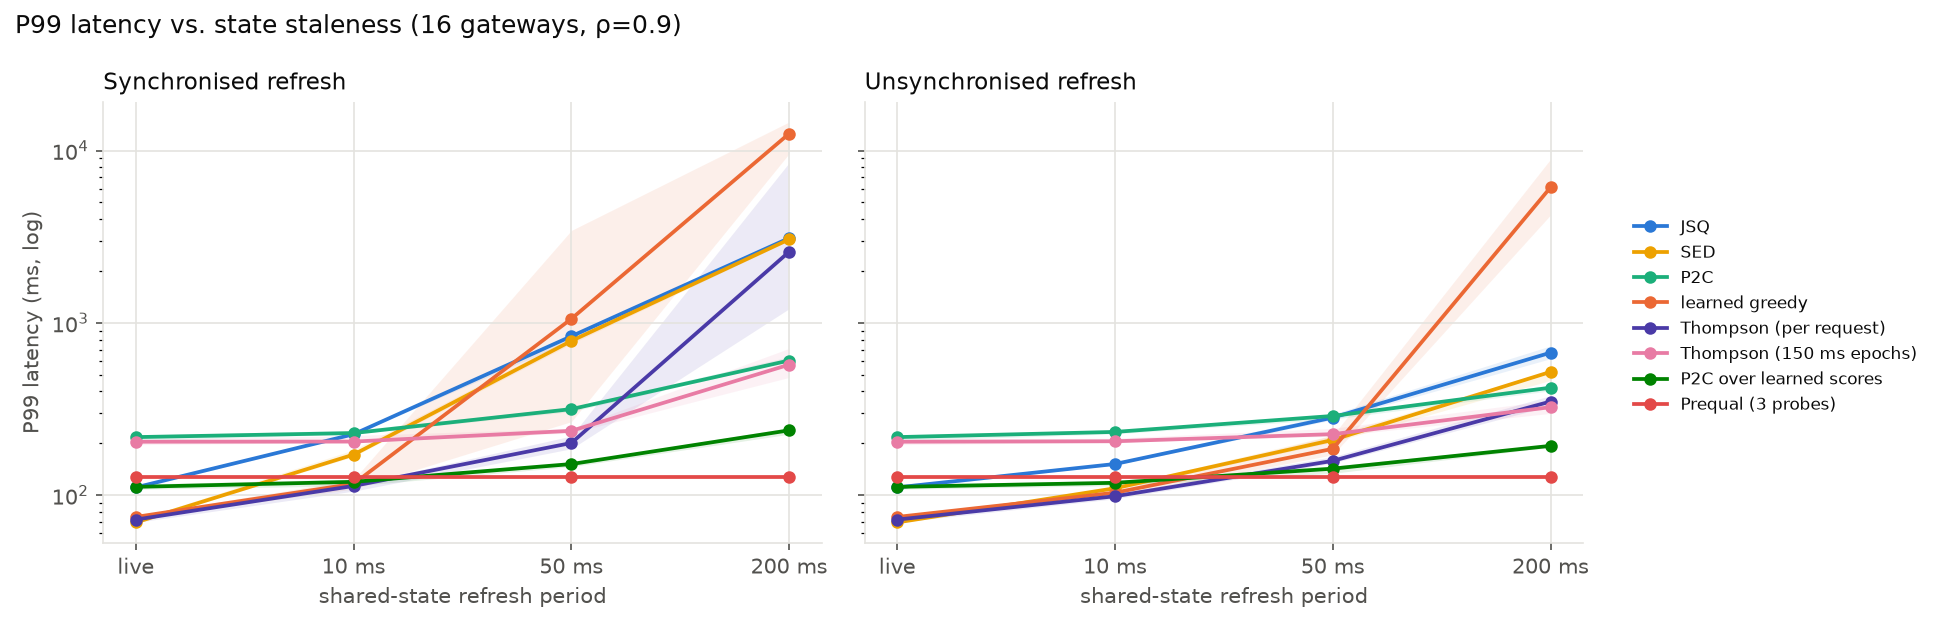
\includegraphics[width=\textwidth]{fig1_p99_vs_staleness.png}
  \caption{P99 latency against snapshot staleness, with 16 gateways and $\rho=0.9$. Left: every gateway
  refreshes at the same instants. Right: each gateway refreshes on its own phase.}
  \label{fig:staleness}
\end{figure*}

\Cref{fig:staleness} (left) shows the synchronised case. With live state,
learned greedy (75\,ms) and TS (72\,ms) match SED, which is told the true
speeds (69\,ms). Once state is stale, argmin routing collapses. At 50\,ms,
JSQ reaches 836\,ms and \emph{learned greedy 1{,}055\,ms}. At 200\,ms they
reach 3.1\,s and 12.5\,s. The herding index confirms these are stampedes: at
50\,ms it is 30.8 for JSQ, 9.4 for greedy and 8.1 for TS, against 2.5 for P2C
and 2.0 for P2C-L. Per-request TS holds up to 50\,ms (201\,ms) but collapses at
200\,ms (2.6\,s).

\paragraph{Desynchronising refresh is not enough.} Unsynchronised refresh
(\cref{fig:staleness}, right) removes most of the classic herding: at 50\,ms
JSQ improves from 836 to 282\,ms. Learned greedy, however, still reaches
6.1\,s at 200\,ms, and 7.0\,s with 64 gateways at 50\,ms. P2C-L stays at
142--193\,ms across all staleness levels.

\subsection{Scaling the number of gateways}
\begin{figure*}[t]
  \centering
  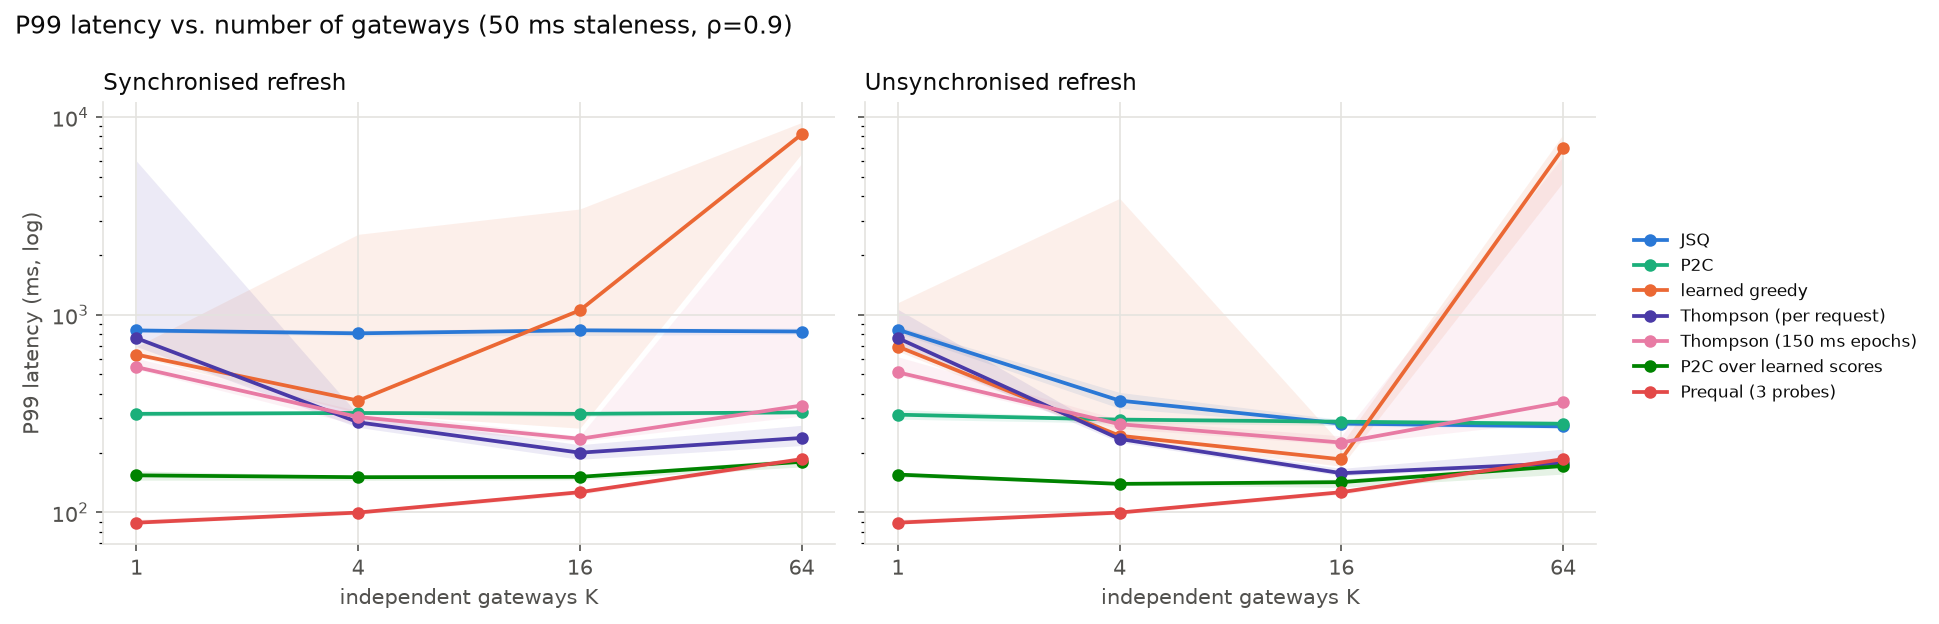
\includegraphics[width=\textwidth]{fig2_p99_vs_dispatchers.png}
  \caption{P99 latency against the number of gateways at 50\,ms staleness.}
  \label{fig:gateways}
\end{figure*}
\Cref{fig:gateways} separates the two herding mechanisms from
\cref{sec:mechanism}.
\begin{itemize}
\item \textbf{Within a gateway.} With one gateway, learned greedy (630\,ms)
  and TS (763\,ms) are poor, because all of that gateway's requests between
  refreshes go to one backend. Local correction fixes this: greedy+lc reaches
  100\,ms and TS+lc 103\,ms.
\item \textbf{Across gateways.} Local correction cannot see other gateways'
  sends, so greedy+lc degrades to 8.1\,s at $K{=}64$. TS instead
  \emph{improves} from $K{=}1$ to $K{=}16$ (763 to 201\,ms): independently
  trained posteriors disagree, which decorrelates the gateways.
\item \textbf{Learned power-of-$d$.} P2C-L varies only between 151 and
  180\,ms across $K$, as \cref{prop:cap} predicts.
\end{itemize}

\subsection{Control intervals are hidden staleness}
\label{sec:eval-epoch}
TS-epoch recomputes weights every control interval and routes by those weights
in between, as learned-router control planes commonly do. Even with
\emph{live} backend state, its P99 is 137, 149, 204 and 800\,ms for intervals of
10, 50, 150 and 500\,ms, against 72\,ms for per-request TS. The interval acts
as a second staleness knob, on top of the state refresh period: with 50\,ms
state staleness the same intervals give 156 to 1{,}107\,ms. TS-epoch also
herds at scale (348\,ms at 64 gateways, with an IQR reaching 5.8\,s).

\subsection{Gray failure}
\begin{figure*}[t]
  \centering
  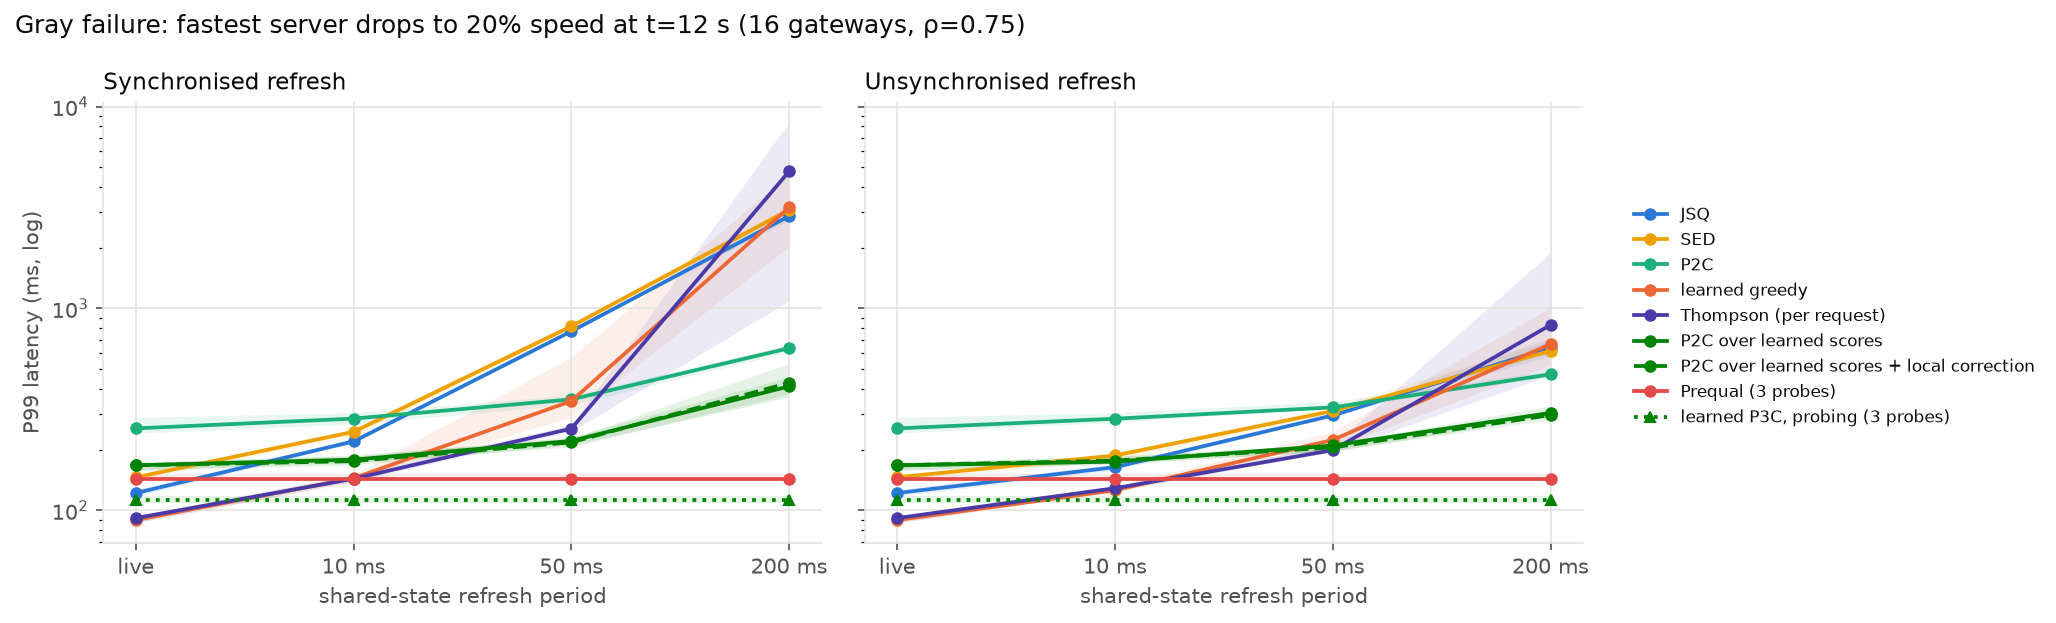
\includegraphics[width=\textwidth]{fig5_gray_failure.png}
  \caption{Gray failure: the fastest backend drops to 20\% speed at $t{=}12$\,s ($\rho=0.75$, 16 gateways).}
  \label{fig:gray}
\end{figure*}
When a backend slows down without announcement (\cref{fig:gray}), policies that
trust nominal speeds keep feeding it. SED rises from 69\,ms in steady state to
146\,ms with live state. Learned models notice the slowdown from latency
alone: greedy reaches 89\,ms and TS 91\,ms. Once state is stale, the herding
results repeat. With synchronised refresh at 200\,ms, greedy reaches 3.2\,s
and TS 4.8\,s, while P2C-L stays at 411\,ms.

\subsection{Probe cost, and learning versus probing}
\begin{figure*}[t]
  \centering
  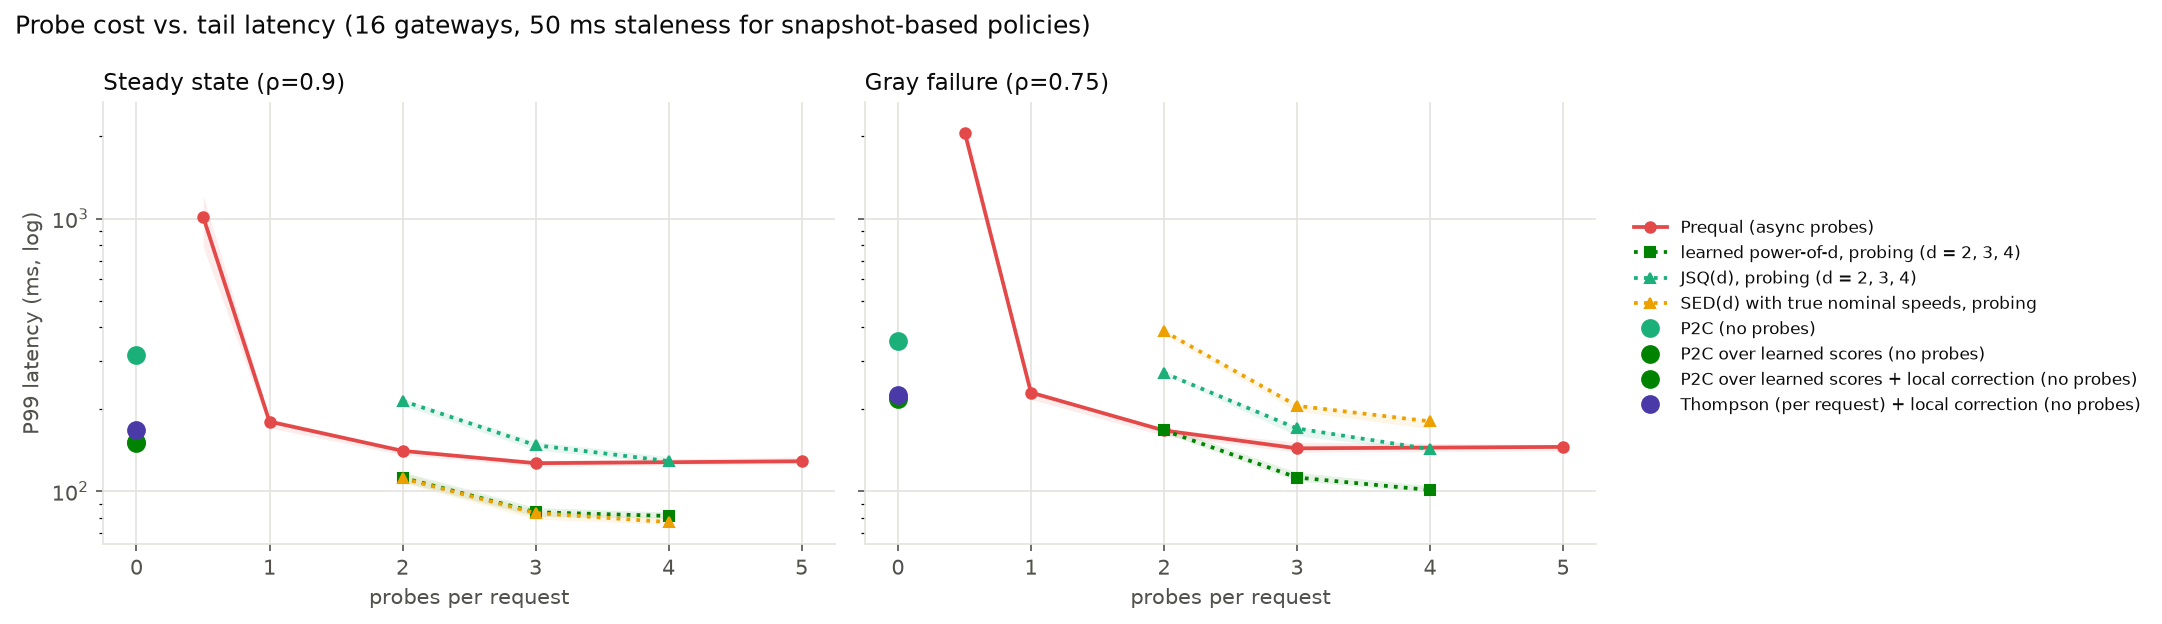
\includegraphics[width=\textwidth]{fig7_probe_frontier.png}
  \caption{P99 latency against probes per request (16 gateways). Snapshot-based policies (at $x{=}0$) use
  50\,ms-stale shared state.}
  \label{fig:frontier}
\end{figure*}
\Cref{fig:frontier} compares policies at equal probe cost. It also separates
what learning contributes from what probing contributes.
\begin{itemize}
\item \textbf{Zero probes.} P2C-L (151\,ms steady, 221\,ms gray) beats
  Prequal limited to one probe per request (180 and 230\,ms). Prequal
  degrades sharply below one probe per request (1.0\,s at 0.5).
\item \textbf{Equal budgets.} At 3 probes per request, P3C-L-probe gets
  84\,ms against Prequal's 127\,ms in steady state, and 112 against 144\,ms
  under gray failure.
\item \textbf{Learning versus probing.} In steady state, P3C-L-probe matches
  SED(3), which is \emph{told} the true speeds (84 vs.\ 83\,ms), and beats
  JSQ(3), which ignores heterogeneity (147\,ms). So the learned model recovers
  the oracle's knowledge. Under gray failure the oracle's knowledge goes stale:
  SED(3) rises to 206\,ms while P3C-L-probe holds at 112\,ms.
\end{itemize}
Learning therefore pays off when server speeds are unknown or drifting, and
the sampling step supplies robustness to staleness.

Probing policies do not scale equally. From 1 to 64 gateways, Prequal's P99
rises from 89 to 186\,ms and P3C-L-probe's from 82 to 99\,ms. P3C-L-probe
degrades with $K$ because each gateway learns from $1/K$ of the traffic.

\subsection{Robustness}
\paragraph{Heavy-tailed service.} We use lognormal service times with
coefficient of variation 2 and 4, at 50\,ms staleness with synchronised
refresh. Every policy's tail grows. The ranking among snapshot policies holds:
P2C-L gets 325 and 772\,ms, against 1{,}055 to 8{,}342\,ms for greedy. Among
probing policies, however, the oracle SED(3) now leads (186 and 419\,ms),
ahead of P3C-L-probe (190 and 483\,ms) and Prequal (262 and 598\,ms). Noisy
service slows learning; this is the cost of not knowing the speeds.

\paragraph{Bursty arrivals.} We add a two-state Markov-modulated arrival
process with $\pm25\%$ rate swings at $\rho=0.75$. The conclusions are
unchanged (\texttt{research/results/summary.md}).

\paragraph{Load.} From $\rho=0.5$ to $0.95$, P2C-L rises from 70 to 191\,ms
and P3C-L-probe from 45 to 124\,ms. Learned greedy becomes unstable from
$\rho=0.9$ (3.9\,s at 0.95).

\subsection{Real-system validation}
\label{sec:eval-real}
\TODO{Fill from research/results/realsys.csv: K gateway processes (src/gateway.py)
sharing one Redis, 8 FIFO backend processes, open-loop Poisson load; 5$\times$
slower time scale than the simulator; nominal $\rho=0.8$.}

% ---------------------------------------------------------------------------
\section{Related Work}
\TODO{Author must complete after reading: multi-dispatcher load balancing with
stale or local information \citep{zhou2020multidispatcher,goren2021stochastic};
old-information results \citep{mitzenmacher2000old,dahlin2000stale};
power of $d$ choices \citep{mitzenmacher2001power}; replica selection \citep{c3nsdi2015};
probing \citep{prequal2024}; learned and LLM routers \citep{lodestar2026,llmd,vllmrouter};
multi-player bandits \citep{multiplayerbandit2025}.
State precisely how each differs from this work.}

\section{Limitations}
Our backends are single-server FIFO queues and the learned model has two
features; real backends are multi-core, and richer context may change the
ranking among learned policies. The Prequal baseline is our re-implementation
from the paper's description and is tuned in its favour, but it is not the
production system. Our probing variants probe synchronously; with sub-millisecond
service times the probe round-trip, which Prequal avoids, would matter more
than in our setting. The prototype validation uses a 5$\times$ slower time scale
than the simulator so that Python processes keep up.

\section{Conclusion}
Horizontally scaled learned routers are exposed to herding in two ways.
Within a gateway, requests pile onto one backend between refreshes. Across
gateways, models trained on similar data reach the same answer. Control
intervals add staleness of their own. The remedy is cheap: keep the learned
score for \emph{ranking}, but let random candidate sampling decide
\emph{which} backends are ranked. This bounds any backend's share of traffic
independently of how stale or how widely shared the state is, and it keeps
the benefit of learning when server speeds are unknown or change.

\bibliographystyle{plainnat}
\bibliography{refs}
\end{document}
